% Some commands used in this file
\newcommand{\package}{\emph}

\chapter{Introduction}
\label{chap:introduction}

In the study of astrophysical entities, accretion shocks are a fairly commonly encountered physical phenomena. In particular, standing accretion shocks (SAS) are part of the theory behind core-collapse supernovae, with an instability (SASI) described by Blondin et al.~\cite{Blondin2003} being proposed as a possible mechanism for driving the explosive evolution of these physical systems. This instability occurs because of the spherical nature of the system, with the effects of perturbations to the symmetry of the shock being trapped in the interior subsonic region and producing feedback loops which further perturb the shock front.

To gain a better understanding of the underlying mechanisms of this instability, Foglizzo~\cite{Foglizzo2009} and Sato et al.~\cite{Sato2009} (hereafter referred to together as FS) proposed and studied a simple toy problem, the details of which are presented in Section \ref{sec:toyProblem}. Using this simple set-up they showed evidence for a coupled advective-acoustic cycle between the stationary shock front and an interior decelerating potential step that is intended to model the effects of matter settling onto the surface of the accreting object. This potential step is of particular note in that it gives rise to non-trivial steady state flows which may not be adequately simulated by standard numeric schemes.

For this thesis, therefore, a well-balanced method for simulating steady states in the presence of external potential fields, extended from that developed by K\"appeli and Mishra~\cite{Kappeli2014} (hereafter referred to as KM), was applied to the aforementioned toy problem with an eye to higher dimensional simulations of the SASI scenario using circular and spherical geometries. The mathematical theory of fluid flow and associated steady states is briefly outlined in Section~\ref{sec:euler} while an overview of the numerical method and well-balanced scheme used for this thesis is given in Section~\ref{sec:numerics}. Details of the set-up and results of numerical simulations carried out using our implementation of the well-balanced scheme are presented in Chapter~\ref{chap:results}.


\section{Euler Equations}
\label{sec:euler}

The time evolution of the dynamics of fluids can be described by systems of balance laws. For inviscid fluids, this system is given by the well-known Euler equations with source terms, which mathematically represent the physical conservation of mass, momentum, and energy. They are given here following the notation of KM as
\begin{subequations} \label{eq:eulerFull}
\begin{align}
\frac{\partial{\rho}}{\partial{t}} &+ \nabla \cdot (\rho \mathbf{v}) = 0, \label{eq:eulerContinuity} \\
\frac{\partial{\rho \mathbf{v}}}{\partial{t}} &+ \nabla \cdot (\mathbf{v} \rho \mathbf{v}) + \nabla p = -\rho \nabla \phi, \label{eq:eulerMomentum} \\
\frac{\partial{E}}{\partial{t}} &+ \nabla \cdot \left[(E+p)\mathbf{v}\right] = -\rho \mathbf{v} \cdot \nabla \phi,  \label{eq:eulerEnergy} 
\end{align}
\end{subequations}
where $\rho$ is the mass density, and $\mathbf{v}$ is the local velocity vector. $E$ is the total energy sum of the internal and kinetic energies given as
\begin{equation}
E=\rho e + \frac{\rho \mathrm{v}^2}{2}.
\end{equation}
An equation of state $p=p(\rho,e)$ must be selected for a given problem to complete the relations between these primitive quanitites. The quantitiy $\phi$ on the right-hand side of the latter two equations represents a potential field, such as gravity, which acts upon the fluid. For our purposes, this potential is assumed to be known, either as a given function, through pre-computation, or by solving for it independently of the other fluid quantities at each time step.

The Euler system of equations can be rewritten in the condensed form of a general balance law as
\begin{equation} \label{eq:euler}
\mathbf{U}_t+\nabla\cdot(\mathbf{F}(\mathbf{U}))=\mathbf{S}(\mathbf{U}),
\end{equation}
where $\mathbf{U}$ is a vector of the conserved quantities, and the vectors $\mathbf{F}$ and $\mathbf{S}$ represent the fluxes and sources of these quanitites in the system.

\subsection{Steady States}

For fluid flows in the presence of an external potential field, non-trivial steady states (also called stationary solutions) can arise. Highly accurate simulations of these stationary solutions are of interest as they allow for accurate reproduction and analysis of subsequent perturbations to the system, which can be quite small and therefore overwhelmed by the truncation error of a less well-resolved scheme.

For a steady state solution the time derivative term is exactly zero and it can be seen that the balance law~\eqref{eq:euler} reduces to a balance between the fluxes and sources as
\begin{equation} \label{eq:balance}
\nabla\cdot(\mathbf{F}(\mathbf{U}))=\mathbf{S}(\mathbf{U}).
\end{equation}
In order to find a unique numerical solution to this balance, some constraint on the thermodynamics of the system must be specified. For example, Bernoulli's principle gives us that the following quantiity should remain constant along streamlines of an isentropic steady flow
\begin{equation}
\frac{\mathrm{v}^2}{2}+\phi+h=\textrm{constant}\equiv b
\end{equation}
where $b$ is referred to as the Bernoulli constant and $h$ is the specific enthalpy
\begin{equation} \label{eq:enthalpy}
h=e+\frac{p}{\rho}.
\end{equation}
This constancy can then be leveraged in a computational scheme to find the unique weak solution for such an isentropic flow.


\section{Numerical Methods}
\label{sec:numerics}

It is well-studied that the non-linear nature of the Euler equations~\eqref{eq:eulerFull} can lead to very complicated flow features, such as turbulence and shocks, even from initially smooth conditions. As such, numerical solutions to these systems can only be found in a weak sense and require not only initial and boundary conditions, but also some other thermodynamic information in order to fix a unique solution. Several options are possible depending on the flow scenario to be modelled, with two important classes comprising constant entropy and constant temeprature flows, i.e.~isentropic and isothermal flows, respectively. Many methods have already been developed and well-studied to resolve such flows in a stable and consistent manner, with the class of finite volume methods (FVM) being one of the most popular for conservation laws.

\subsection{Spatial Discretization}
\label{subsec:space}

Starting in one dimension for simplicity, the Euler equations in the balance law form~\eqref{eq:euler} reduce to
\begin{equation} \label{eq:euler1D}
\frac{\partial \mathbf{U}}{\partial t}+\frac{\partial \mathbf{F}}{\partial x}=\mathbf{S},
\end{equation}
where the vectors of conserved quanitites, and their fluxes and sources are respectively defined as
\begin{equation}
\mathbf{U}=
\begin{bmatrix}
\rho \\ \rho \mathrm{v}_x \\ E
\end{bmatrix}
,\quad \mathbf{F}=
\begin{bmatrix}
\rho \mathrm{v}_x \\ \rho \mathrm{v}_x^2+p \\ (E+p)\mathrm{v}_x
\end{bmatrix}
,\quad \mathbf{S}=
\begin{bmatrix}
0 \\ -\rho \\ -\rho \mathrm{v}_x
\end{bmatrix} \frac{\partial \phi}{\partial x}.
\end{equation}
It is also useful to define a vector of primitive variables $\mathbf{w}=[p,\ \mathrm{v}_x,\ T]^T$. While the methods used here are generally applicable to any choice of the equation of state, the ideal gas law will be assumed here as an example for the derivations. It is given by
\begin{equation}
p=\rho e(\gamma-1),
\end{equation}
where the adiabatic index $\gamma=C_p/C_v$ is the ratio of specific heats at constant pressure and volume, respectively.

A typical FVM discretizes the domain into small cells (i.e. volumes) which in 1D can be denoted $I_i=[x_{i-1/2},x_{i+1/2}]$ and for simplicity will be assumed to be of unform size $\Delta x=x_{i+1/2}-x_{i-1/2}$. The cell averages of the conserved quantities are then evolved in time by computing their fluxes at all of the faces between adjacent volumes. As the values in adjacent cells differ in general, a Riemann problem arises at each cell interface, which can then be solved to obtain the fluxes. Exact solutions are possible, and are the basis of the so-called Godunov schemes~\cite{Godunov1959}, but usually the computational effort is saved by using an approximate solution, such as from a Roe~\cite{Roe1981}, Rusanov~\cite{Rusanov1961}, or HLLC~\cite{Toro1994} solver, as the remainder of the method will be itself only approximate due to truncation error.

Up to second-order accuracy the cell average value is equivalent to the value at the cell centre and so we will treat the two as interchangeable in the following, as only first- and second-order accuracy will be explored. With this, an FVM then also requires one to specifiy a reconstruction scheme to extend these values stored at the cell centres to the cell faces to obtain the Riemann problem at that interface. A piecewise constant reconstruction, where the cell average value is simply used also at the interface, is the simplest such scheme but gives only first-order accuracy.

Second-order accuracy can be achieved by computing the gradient at each cell centre and using that to linearly extrapolate to the cell faces. However, this method generally gives rise to spurious oscillations in the resulting solutions, particularly near sharp flow features such as shock fronts. To counter this, most such schemes limit the gradient in areas of rapid change, reducing the local order of accuracy towards first-order. These limited schemes are referred to as total variation diminishing (TVD) and various slope limiter functions, such as those developed by Barth and Jespersen~\cite{Barth1989}, Venkatakrishnan~\cite{Venkatakrishnan1993,Venkatakrishnan1995}, or Michalak and Gooch~\cite{Michalak2008}, can be used.

\subsection{Well-Balanced Reconstruction}
\label{subsec:wellBalanced}

Standard reconstructions as outlined above do not generally preserve equilibrium states exactly, but merely converge towards the precise stationary solution with increasing grid resolution. Particularly for small perturbations, this global error can dominate small features, which then require prohibitvely small cell sizes to be adequately resolved. It is therefore desirable to develop a scheme for which the flux and source terms of~\eqref{eq:balance} cancel each other exactly for an equilibrium stationary solution. Such a method has been developed for hydrostatic flows by KM, termed a well-balanced scheme, and the salient results of their derivations are here reproduced and extended to non-hydrostatic equilibria. For simplicity, the concrete case of an isentropic flow will be used here, although it is stressed that the fundamental ideas of the following well-balanced scheme are equally applicable to other thermodynamic conditions.

We will use the thermodynamic definitions of the specific enthalpy~\eqref{eq:enthalpy} and specific energy
\begin{equation}
e=\frac{p}{(\gamma-1)\rho},
\end{equation}
along with the polytropic form of the equation of state
\begin{equation}
p=p(K,\rho)=K\rho^{\gamma},
\end{equation}
where $K=K(s)$ is only a function of the entropy $s$, and so is constant for isentropic flows. From this, the Bernoulli constant can be recast in terms of a single unknown variable, in this case the mass density $\rho(x)$, as
\begin{equation}
\frac{1}{2}\frac{m^2}{\rho^2}+\frac{\gamma}{\gamma-1}K\rho^{\gamma-1}+\phi=b, \label{eq:bernoulli}
\end{equation}
where the continuity equation~\eqref{eq:eulerContinuity} for a steady state shows that the mass flux $m=\rho \mathrm{v}_x$ is also constant.

All of the constant values in~\eqref{eq:bernoulli} can be computed for a given cell $i$ and timestep $n$ using the stored cell-centred values, and then the known variation in $\phi(x)$ can be leveraged to compute the value of $\rho(x)$ throughout the cell as
\begin{equation}
\frac{1}{2}\left(\frac{m_i^n}{\rho_{0,i}^n(x)}\right)^2+\frac{\gamma}{\gamma-1}K_i^n\rho_{0,i}^n(x)^{\gamma-1}+\phi(x)=b_i^n.
\end{equation}
This computaton gives the extrapolated values that $\rho(x)$ would have in the area around the $i\textrm{-th}$ cell for a steady state flow, and so is termed the equilibrium value and denoted with a `$0$' subscript. If the potential $\phi(x)$ is a known function, then this allows $\rho_0(x)$ to be computed everywhere in the cell neighbourhood; however, if $\phi(x)$ is also given only discretely at the cell centres, perhaps becuase it is itself computed numerically in a separate calculation, then it must be interpolated to the desired reconstruction points (i.e. the cell faces) in order to compute $\rho_0$ there. A second order accurate piece-wise linear interpolation is generally sufficient, provided the underlying $\phi(x)$ is a continuous function.

Equilibrium reconstruction values for the primitive variables can then be obtained from the computed $\rho_{0,i}^n$, giving
\begin{equation} \label{eq:primitives1D1}
\mathbf{w}_{i-1/2+}^n=
\begin{bmatrix}
p_{0,i}^n(x_{i-1/2}) \\ \mathrm{v}_{x,0,i}^n(x_{i-1/2}) \\ T_{0,i}^n(x_{i-1/2})
\end{bmatrix}
\quad \textrm{and} \quad \mathbf{w}_{i+1/2-}^n=
\begin{bmatrix}
p_{0,i}^n(x_{i+1/2}) \\ \mathrm{v}_{x,0,i}^n(x_{i+1/2}) \\ T_{0,i}^n(x_{i+1/2})
\end{bmatrix},
\end{equation}
as inputs to the chosen Riemann solver at the cell interfaces.

\subsection{Discretization of Source Terms}
\label{subsec:sources}

To achieve exact balancing of the source and flux terms, we require that the diexcretizations are not only consistent, but also that the constants and higher order terms of the Taylor expansions precisely match. Following KM, the definitions used for the source terms are
\begin{align}
S_{\rho \mathrm{v},i}^n&=\frac{\left[\rho_{0,i}^n(\mathrm{v}_{x,0,i}^n)^2+p_{0,i}^n\right]_{x_{i-1/2}}^{x_{i+1/2}}}{\Delta x}=-\int\limits_{x_{i-1/2}}^{x_{i+1/2}}\rho \frac{\partial \phi}{\partial x}\textrm{d}x+O\left(\Delta x^2\right), \label{eq:momentumSource} \\
S_{E,i}^n&=-\rho \mathrm{v}_{x,i}^n\frac{\phi_{i+1}-\phi_{i-1}}{2\Delta x}=-\int\limits_{x_{i-1/2}}^{x_{i+1/2}}\rho \mathrm{v}_x \frac{\partial \phi}{\partial x}\textrm{d}x+O\left(\Delta x^2\right), \label{eq:energySource}
\end{align}
where the notation $\left[f(x)\right]_a^b\equiv f(x=b)-f(x=a)$ is used for the momentum source term.

Both of these are spatially second-order accurate approximations of the source terms in~\eqref{eq:euler1D}, but are specifically chosen such that the higher order error terms will precisely cancel those of the corresponding numerical flux approximations for equilibirum flows. Together these discretizations give the source vector
\begin{equation}
\mathbf{S}_i^n=
\begin{bmatrix}
0 \\ S_{\rho \mathrm{v},i}^n \\ S_{E,i}^n
\end{bmatrix}.
\end{equation}
Combining the above source vector with the primitives of~\eqref{eq:primitives1D1} gives a well-balanced scheme which will exactly preserve a given equilibrium state to machine precision, provided the potential is either fully known or defined discretely on the given grid. The scheme will, however, only model perturbations of the equilibrium with first-order accuracy in space.

\subsection{Extension to Second Order}
\label{subsec:secondOrder}

As first-order accuracy is generally insufficient for most practical problems of interest, the next step is to extend the method to achieve second-order accuracy for perturbations while maintaining the well-balanced properties for the underlying equilibrium. As alluded to at the end of section~\ref{subsec:space}, a TVD slope-limited linear extrapolation is used to improve the reconstruction of the primitives to the cell faces. Using `$q$' as a placeholder for any of the required primitve variables, we thus define a second-order equilibrium-preserving reconstruction $q_i(x)$ in the $i\textrm{-th}$ cell as
\begin{equation}
q_i(x)=q_{0,i}(x)+Dq_{1,i}(x-x_i),
\end{equation}
where $q_{0,i}(x)$ is the same equilibrium reconstruction computed previously, and $Dq_{1,i}$ is the limited gradient of the perturbation term for the primitive variable within the cell centred at $x_i$. This perturbation term is denoted by a subscript `$1$' as $q_{1,i}(x)$ and is given as
\begin{equation}
q_{1,i}(x)=q(x)-q_{0,i}(x).
\end{equation}
It represents the difference between the current solution value $q(x)$ and the purely equilibrium extrapolated values computed for the local cell, and therefore models any perturbations of the flow away from the underlying steady state. Note that when evaluated at the $i\textrm{-th}$ cell centre one will always get $q_{1,i}(x_i)=q_i-q_{0,i}(x_i)=0$, as the equilibrium reconstruction is computed using the solution values at that cell centre and so will always precisely match the current solution at that location. The illustration in Fig.~\ref{fig:Kappeli1} visually shows how the relationship between $p(x)$, $p_{0,i}(x)$, and $p_{1,i}(x)$ might look for a hypothetical pressure curve containing a clearly non-zero deviation from the equilibrium state.
\begin {figure}
\centering
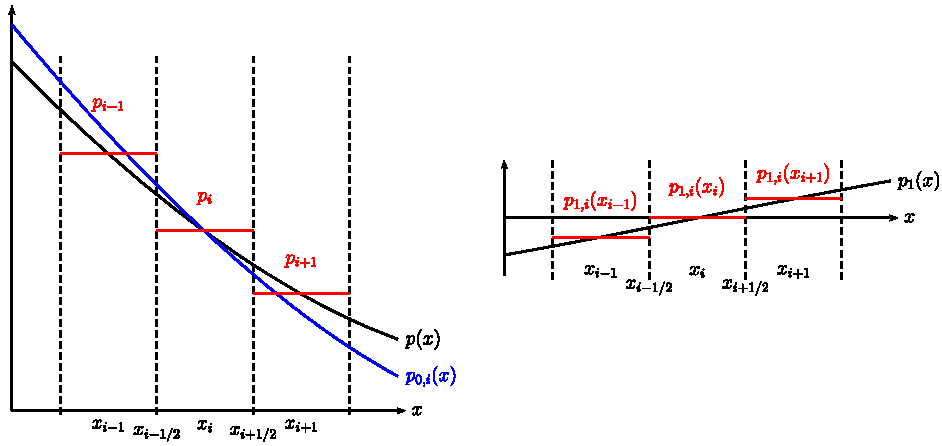
\includegraphics[width=13cm]{figures/Kaeppeli1}
\caption{This image is taken directly from KM~\cite{Kappeli2014}. In the left pane, the reconstruction begins with only the cell average values, shown in red, which to second-order accuracy are equal to the current solution $p(x)$, shown in black, evaluated at the cell centres. The blue line shows the value of the equilibrium $p_{0,i}(x)$ extrapolated from the constant values computed at the $i\textrm{-th}$ cell centre. Subtracting the blue line from the black line then gives the perturbation function $p_{1,i}(x)$ in the right pane.}
\label{fig:Kappeli1}
\end{figure}

Because the current solution $q(x)$ is known only at the cell centres, the required local slope is determined by computing the value of $q_{0,i}(x)$ not only at the cell faces as in the first-order case, but also at the neighbouring cell centres. These extrapolated values are then subtracted from the known solution values at those cell centres as
\begin{equation}
q_{1,i}(x_{i-1})=q_{i-1}-q_{0,i}(x_{i-1})\quad \textrm{and}\quad q_{1,i}(x_{i+1})=q_{i+1}-q_{0,i}(x_{i+1}).
\end{equation}
The limited slope can then be computed by applying a TVD limiter funtion to the estimates of the local slope obtained from the neighbouring perturbation values as
\begin{equation}
Dq_{1,i}=\textrm{limiter}\left(\frac{q_{1,i}(x_i)-q_{1,i}(x_{i-1})}{\Delta x},\frac{q_{1,i}(x_{i+1})-q_{1,i}(x_i)}{\Delta x}\right).
\end{equation}
There are many potential choices of limiter function described in the literature, one of the most common and simple of which is the \emph{minmod} limiter, defined as
\begin{equation}
\textrm{minmod}(a,b)=\frac{1}{2}\left(\textrm{sign}(a)+\textrm{sign}(b)\right)\textrm{min}\left(|a|,|b|\right).
\end{equation}
As noted earlier, the perturbation terms will be zero at the current cell centre, and so the final form of the second-order reconstruction simplifies to
\begin{equation} \label{eq:secondOrderReconstruction}
q_i(x)=q_{0,i}(x)+\textrm{limiter}\left(-\frac{q_{1,i}(x_{i-1})}{\Delta x},\frac{q_{1,i}(x_{i+1})}{\Delta x}\right)(x-x_i).
\end{equation}
It is easy to see that for a flow which is already at equilibrium, the equilibrium reconstruction $q_{0,i}(x)$ will be precisely equal to the solution values $q(x)$ at the neighbouring cells, and so the $q_{1,i}(x)$ terms in~\eqref{eq:secondOrderReconstruction} will all be zero by design. Thus, for already steady state flows it reduces to the first-order scheme previously derived, thereby preserving the equilibrium exactly also for this second-order scheme. The final vectors of primitive values which are input to the Riemann solver are
\begin{align} \label{eq:primitives1D2}
\begin{split}
\mathbf{w}_{i-1/2+}^n&=
\begin{bmatrix}
p_{0,i}^n(x_{i-1/2})+p_{1,i}^n(x_{i-1/2}) \\ v_{x,0,i}^n(x_{i-1/2})+v_{x,1,i}^n(x_{i-1/2}) \\ T_{0,i}^n(x_{i-1/2})+T_{1,i}^n(x_{i-1/2})
\end{bmatrix} \\
&\textrm{and} \\
\mathbf{w}_{i+1/2-}^n&=
\begin{bmatrix}
p_{0,i}^n(x_{i+1/2})+p_{1,i}^n(x_{i+1/2}) \\ v_{x,0,i}^n(x_{i+1/2})+ v_{x,1,i}^n(x_{i+1/2}) \\ T_{0,i}^n(x_{i+1/2})+T_{1,i}^n(x_{i+1/2})
\end{bmatrix}.
\end{split}
\end{align}
The same discretization of the source terms as in~\eqref{eq:momentumSource} and~\eqref{eq:energySource} are used, as they are already second-order accurate and must remain unchanged to preserve the well-balanced property of the reconstruction for equilibrium flows.

\subsection{Time Discretization}
\label{subsec:time}

After specifying a spatial discretization, the system of equations~\eqref{eq:euler} can be written in the semi-discrete form
\begin{equation}
\mathbf{U}_t=\mathbf{R}(\mathbf{U}),
\end{equation}
where $\mathbf{R}$ is a simple notation to represent the residual from the chosen spatial scheme, as outlined above.

The time discretization which is then used to advance the solution is a four-stage, low-storage Runge-Kutta (RK) scheme with the following form
\begin{align}
\begin{split}
\mathbf{U}^{(0)} &\equiv \mathbf{U}^n,\\
\mathbf{U}^{(i)} &= \mathbf{U}^{(0)} + \beta_i \Delta t \mathbf{R} \left(\mathbf{U}^{(i-1)}\right),\qquad i=1,2,3,4,\\
\mathbf{U}^{n+1} &\equiv \mathbf{U}^{(4)},
\end{split}
\end{align}
where $n$ is the global time index, $i$ is the index of the intra-timestep RK stage, and $\Delta t=t^{n+1}-t^n$ is the size of the current time step. The specific time-marching scheme used is described in~\cite{Lallemand1990} and has the coefficients
\begin{equation}
\beta_1=0.11,\quad \beta_2=0.2766,\quad \beta_3=0.5,\quad \beta_4=1.
\end{equation}
Having $\beta_4=1$ ensures that such a scheme is consistent, and having $\beta_3=0.5$ means the method is second-order accurate for both linear and non-linear equations. The values for $\beta_1$ and $\beta_2$ were designed to maxmize the largest stable CFL coefficient, and therefore possible timestep size, when paired with upwind based spatial discretization schemes. According to~\cite{Shu1988} and \cite{Macdonald2003}, having every $\beta_i \geq 0$ also means that the scheme belongs to the desirable class of strong stability preserving (SSP) RK methods.

\subsection{Multiple Spatial Dimensions}
\label{subsec:multiDim}

Extending the method to multiple spatial dimensions is accomplished via a relatively straightforward application of the preceding 1D approach along each additional dimension. It is summarized here for 2D but would progress analgously for 3D cases.

The 1D Euler equation~\eqref{eq:euler1D} is expanded to 2D as
\begin{equation} \label{eq:euler2D}
\frac{\partial \mathbf{U}}{\partial t}+\frac{\partial \mathbf{F}}{\partial x}+\frac{\partial \mathbf{G}}{\partial y}=\mathbf{S},
\end{equation}
where the conserved quantities, fluxes, and source terms are now given by the four-valued vectors
\begin{align}
\begin{split}
\mathbf{U}&=
\begin{bmatrix}
\rho \\ \rho \mathrm{v}_x \\ \rho \mathrm{v}_y \\ E
\end{bmatrix}
,\quad \mathbf{F}=
\begin{bmatrix}
\rho \mathrm{v}_x \\ \rho \mathrm{v}_x^2+p \\ \rho \mathrm{v}_x \mathrm{v}_y \\ (E+p)\mathrm{v}_x
\end{bmatrix}
,\quad \mathbf{G}=
\begin{bmatrix}
\rho \mathrm{v}_y \\ \rho \mathrm{v}_x \mathrm{v}_y \\ \rho \mathrm{v}_y^2+p \\ (E+p)\mathrm{v}_y
\end{bmatrix}, \\
\mathbf{S}&=\mathbf{S}_x+\mathbf{S}_y=
\begin{bmatrix}
0 \\ -\rho \\ 0 \\ -\rho \mathrm{v}_x
\end{bmatrix} \frac{\partial \phi}{\partial x} +
\begin{bmatrix}
0 \\ 0 \\ -\rho \\ -\rho \mathrm{v}_y
\end{bmatrix} \frac{\partial \phi}{\partial y},
\end{split}
\end{align}
and $\mathbf{w}=[p,\ \mathrm{v}_x,\  \mathrm{v}_y,\ T]^T$ is the vector of primitive values.

Analgously to the 1D case, one starts by computing the equilibrium constants $b_i^n$, $K_i^n$, and $m_i^n$ at the cell centres and using those to extrapolate the local subcell equilibrium to the cell faces based on the changes in the potential $\phi(x,y)$ from the cell centres to the faces. If $\phi(x,y)$ is known only discretely, then a bilinear interpolation will now be needed to determine its value at the cell faces. The first-order primitive vector of inputs to the Riemann solver are then
\begin{equation} \label{eq:primitives2D1}
\mathbf{w}_{i\mp1/2\pm,j}^n=
\begin{bmatrix}
p_{0,i,j}^n(x_{i\mp1/2},y_j) \\ \mathrm{v}_{x,0,i,j}^n(x_{i\mp1/2},y_j) \\ \mathrm{v}_{y,0,i,j}^n(x_{i\mp1/2},y_j) \\ T_{0,i,j}^n(x_{i\mp1/2},y_j)
\end{bmatrix}
, \quad \mathbf{w}_{i,j\mp1/2\pm}^n=
\begin{bmatrix}
p_{0,i,j}^n(x_i,y_{j\mp1/2}) \\ \mathrm{v}_{x,0,i,j}^n(x_i,y_{j\mp1/2}) \\ \mathrm{v}_{y,0,,ji}^n(x_i,y_{j\mp1/2}) \\ T_{0,i,j}^n(x_i,y_{j\mp1/2})
\end{bmatrix}.
\end{equation}
The source terms can now be split into a sum of components from the individual dimensions, which are then individually specified similarly as in the 1D case, giving
\begin{equation}
\mathbf{S}_{i,j}=\mathbf{S}_{x,i,j}+\mathbf{S}_{y,i,j}=
\begin{bmatrix}
0 \\ S_{x,\rho \textrm{v},i,j} \\ 0 \\ S_{x,E,i,j}
\end{bmatrix} +
\begin{bmatrix}
0 \\ 0 \\ S_{y,\rho \textrm{v},i,j} \\ S_{y,E,i,j}
\end{bmatrix},
\end{equation}
where the momentum source terms are given by
\begin{align}
\begin{split}
S_{x,\rho \textrm{v},i,j}&=\frac{\left[\rho_{0,i,j}^n(\mathrm{v}_{0,i,j}^n)^2+p_{0,i,j}^n\right]_{x_{i-1/2}}^{x_{i+1/2}}}{\Delta x} \quad \textrm{and} \\
S_{y,\rho \textrm{v},i,j}&=\frac{\left[\rho_{0,i,j}^n(\mathrm{v}_{0,i,j}^n)^2+p_{0,i,j}^n\right]_{y_{j-1/2}}^{y_{j+1/2}}}{\Delta y},
\end{split}
\end{align}
and the energy source terms are given by
\begin{equation}
S_{x,E,i,j}^n=-\rho \mathrm{v}_{x,i,j}^n\frac{\phi_{i+1,j}-\phi_{i-1,j}}{2\Delta x} \quad \textrm{and} \quad S_{y,E,i,j}^n=-\rho \mathrm{v}_{y,i,j}^n\frac{\phi_{i,j+1}-\phi_{i,j-1}}{2\Delta y}.
\end{equation}
These source discretizations are again second-order accurate as in the 1D case, and combined with~\eqref{eq:primitives2D1} they give a scheme which is precisely equilibrium preserving but only first-order accurate for modelling deviations from the steady state.

This can then be improved to second-order by proceeding dimension-by-dimension as in the 1D case and computing the differences between the local equilibrium reconstruction evaluated at the neighbouring cell centres and the solution values there, to create a local subcell reconstruction of the perturbations using a gradient-limited linear approximation. This leads to the following second-order accurate primitve vectors
\begin{align} \label{eq:primitives2D2}
\begin{split}
\mathbf{w}_{i\mp1/2\pm,j}^n&=
\begin{bmatrix}
p_{0,i,j}^n(x_{i\mp1/2},y_j)+p_{1,i,j}^n(x_{i\mp1/2},y_j) \\ \mathrm{v}_{x,0,i,j}^n(x_{i\mp1/2},y_j)+\mathrm{v}_{x,1,i,j}^n(x_{i\mp1/2},y_j) \\ \mathrm{v}_{y,0,i,j}^n(x_{i\mp1/2},y_j)+\mathrm{v}_{y,1,i,j}^n(x_{i\mp1/2},y_j) \\ T_{0,i,j}^n(x_{i\mp1/2},y_j)+T_{1,i,j}^n(x_{i\mp1/2},y_j)
\end{bmatrix} \quad \textrm{and} \\
\mathbf{w}_{i,j\mp1/2\pm}^n&=
\begin{bmatrix}
p_{0,i,j}^n(x_i,y_{j\mp1/2})+p_{1,i,j}^n(x_i,y_{j\mp1/2}) \\ \mathrm{v}_{x,0,i,j}^n(x_i,y_{j\mp1/2})+\mathrm{v}_{x,1,i,j}^n(x_i,y_{j\mp1/2}) \\ \mathrm{v}_{y,0,,ji}^n(x_i,y_{j\mp1/2})+\mathrm{v}_{y,1,,ji}^n(x_i,y_{j\mp1/2}) \\ T_{0,i,j}^n(x_i,y_{j\mp1/2})+T_{1,i,j}^n(x_i,y_{j\mp1/2})
\end{bmatrix}.
\end{split}
\end{align}
